\section{Численные алгоритмы решения прямых задач сложного теплообмена}
\label{sec:ch4/sec1}

\subsection{Метод Ньютона для стационарной модели}
\label{subsec:ch4/sec1/stationary}
Краевая задача сложного теплообмена
имеет вид (см.\ раздел~\ref{subsec:ch1/sec3/state})

\begin{equation}
    \label{eq:4_1:1}
    -a \Delta \theta+b \kappa_{a}| \theta|^{3} \theta =
    b \kappa_{a} \varphi,
\end{equation}
\begin{equation}
    \label{eq:4_1:2}
    -\alpha \Delta \varphi+\kappa_{a} \varphi =
    \kappa_{a}|\theta|^{3} \theta,
\end{equation}
\begin{equation}
    \label{eq:4_1:3}
    a \frac{\partial \theta}{\partial n}
    +\left.\beta\left(\theta-\theta_{b}\right)\right|_{\Gamma}=0,
    \quad \alpha \frac{\partial \varphi}{\partial n}
    +\left.\gamma\left(\varphi-\theta_{b}^{4}\right)\right|_{\Gamma}=0.
\end{equation}
Основную сложность при численном решении прямой задачи представляет нелинейность
по температурному полю, которое входит в систему
дифференциальных уравнений в четвёртой степени.

Метод простой итераций успешно применяется для решения задач в двумерной области.
К примеру, он был использован в работах~\cite{Kovtanyuk2015,astrakhantseva2014numerical}.
Однако, в трёхмерной области этот метод демонстрирует недостаточную скорость сходимости,
что приводит к долгим итерационным процессам и увеличению вычислительных затрат.
Эффективное решение прямых граничных задач необходимо для решения задач оптимального управления,
так как алгоритмы оптимизации подразумевают решение прямой задачи на каждой итерации.


Вместо метода простой итераций для решения сложных задач оптимального управления
температурой может быть применен метод Ньютона.
Метод Ньютона является одним из наиболее эффективных методов решения нелинейных уравнений.
Он использует локальную аппроксимацию функции в виде касательной плоскости
и обновляет решение на основе градиента и гессиана функции.
Этот метод обычно обеспечивает быструю сходимость и применяется
для решения прямых задач сложного теплообмена.

Метод Ньютона является усовершенствованным вариантом метода простой итерации,
в котором нелинейное слагаемое $|\theta|^3 \theta$ аппроксимируется
выражением $\widetilde{\theta}^4+4 \widetilde{\theta^3}(\theta-\widetilde{\theta})$,
где $\widetilde{\theta}$ -- приближение для температуры на предыдущей итерации.
Эта аппроксимация обеспечивает более точное решение и быструю сходимость,
что делает метод Ньютона более эффективным для
решения задач с высокой степенью нелинейности.
В результате модифицированная система уравнений примет следующий вид:

\begin{equation}
    \tag{L1}
    \label{eq:L1}
    \begin{gathered}
        -a \Delta \theta+b \kappa_{a}\left(\left(4 \widetilde{\theta}^{3}
        \theta-3 \widetilde{\theta}^{4}\right)-\varphi\right)=0,\\
        \quad-\alpha \Delta \varphi
        +\kappa_{a}\left(\varphi
        -\left(4 \widetilde{\theta}^{3}
        \theta-3 \widetilde{\theta}^{4}\right)\right)=0;
    \end{gathered}
\end{equation}
\begin{equation}
    \tag{L2}
    \label{eq:L2}
    a \frac{\partial \theta}{\partial n}
    +\left.\beta\left(\theta-\theta_{b}\right)\right|_{\Gamma}=0,
    \quad \alpha \frac{\partial \varphi}{\partial n}
    +\left.\gamma\left(\varphi-\theta_{b}^{4}\right)\right|_{\Gamma}=0.
\end{equation}

Монотонная сходимость метода Ньютона является важным свойством,
которое позволяет обеспечить устойчивость итерационного процесса
и успешное решение эллиптических уравнений
с монотонным и выпуклым нелинейным слагаемым.
В литературе было проведено множество исследований, направленных
на изучение сходимости метода Ньютона для таких уравнений.

В частности, в работах~\cite{Mukhamadiev1971, Schryer1971} были представлены
результаты анализа монотонной сходимости метода Ньютона для эллиптического
уравнения с монотонным и выпуклым нелинейным слагаемым.
Результаты этих исследований показывают, что метод Ньютона обладает
хорошими свойствами сходимости и может быть применен для решения
задач оптимального управления в моделях сложного теплообмена.

%\subsection{Квазистационарные и квазилинейные модели}
%\label{subsec:ch4/sec1/quasi}
%
%\textbf{Квазистационарная модель} радиационного и диффузионного теплообмена в ограниченной области
%$\Omega \subset \mathbb{R}^{3}$ с границей $\Gamma=\partial \Omega$
%в разделе~\ref{sec:ch2/sec3} представлена следующим образом
%
%\begin{align*}
%    & \frac{\partial \theta}{\partial t} - a \Delta \theta
%    + b \kappa_{a} \left(|\theta| \theta^{3}-\varphi\right) = 0,\\
%    & - \alpha \Delta \varphi
%    + \kappa_{a} \left(\varphi-|\theta| \theta^{3}\right) = 0, \\
%    \quad x \in \Omega, \quad 0 < t < T;
%    a \left(\partial_{n} \theta+\theta\right)=r, \\
%    \quad \alpha\left(\partial_{n} \varphi
%    + \varphi\right) = u \text { на } \Gamma;
%    \left.\theta\right|_{t=0} = \theta_{0}.
%\end{align*}
%
%
%
%Квазистационарная модель радиационного и диффузионного теплообмена в ограниченной области
%$\Omega \subset \mathbb{R}^{3}$ с границей $\Gamma=\partial \Omega$ в разделе~\ref{sec:ch3:sec3}
%\begin{gather*}
%    \sigma \partial \theta / \partial t-\operatorname{div}(k(\theta) \nabla \theta)
%    -\beta \varphi=u_{1} \chi, \\
%    \quad-\operatorname{div}(\alpha \nabla \varphi)+\beta \varphi= u_{2} \chi, \\
%    k(\theta) \partial_{n} \theta+\left.\gamma
%    \left(\theta-\theta_{b}\right)\right|_{\Gamma}=0,
%    \quad \alpha \partial_{n} \varphi +
%    \left.0.5 \varphi\right|_{\Gamma}=0,\left.\quad \theta\right|_{t=0}=\theta_{0}.
%        \quad x \in \Omega, \quad 0<t<T, \\
%\end{gather*}
%

\subsection{Примеры численного решения краевой задачи \eqref{eq:4_1:1}--\eqref{eq:4_1:3}}
\label{subsec:ch4/sec1/boundary}


Первым этапом решения задачи методом конечных элементов будет вывод слабой формулировки для
линеаризованной модели.
Для этого умножим уравнения~\eqref{eq:L1} на соответствующие тестовые функции
$v, \psi \in H^1(\Omega)$ и применим формулу Грина.
Учитывая краевые условия~\eqref{eq:L2},
получим вариационные равенства $\forall v, \psi \in H^1(\Omega)$:
\begin{equation*}
    \begin{aligned}
        & a( \nabla \theta, \nabla v ) + \int_\Gamma \beta \theta v d\Gamma
        + \left(b \kappa_a (\left(4 \widetilde{\theta}^{3}
        \theta-3 \widetilde{\theta}^{4}\right) - \varphi ), v\right)
        = \int_\Gamma \beta \theta_b v d\Gamma,
        \\
        & \alpha (\nabla \varphi,\nabla \psi)
        + \int_{\Gamma_0 \cup \Gamma_2} \gamma \varphi v d\Gamma
        + \left( (\kappa_a (\varphi - \left(4 \widetilde{\theta}^{3}
        \theta-3 \widetilde{\theta}^{4}\right)), \psi\right)
        = \int_{\Gamma} \gamma \theta_b^4 \psi d\Gamma.
    \end{aligned}
\end{equation*}

\textbf{Пример 1} (двумерная область).
Положим $\Omega=\{(x,y),\, 0 \leq x,y \leq 1 \}$.

Метод конечных элементов требует разбиения области $\Omega$ на
конечное число непересекающихся подобластей, называющихся
\textit{конечными элементами}.
Отметим, что большинство современных солверов включают в себя
алгоритмы разбиения области на конечные элементы, а также загрузку
уже разбитых областей.

Определим параметры системы следующим образом.
$a = 0.6$,
$\alpha = 0.333$,
$k_a = 1$,
$b = 0.025$,
$\beta = 1$,
$\gamma = 0.8 \cos\left(\frac{\pi}{2} y\right) + 0.5$,
$\theta_b = 0.1 + y / 2$.
Начальное приближение для функций $\theta$ и $\varphi$ выбрано нулевым.
Состояние, полученное за три итерации при данных параметрах представлено
на рисунке~\ref{fig:4_1:boundary}.
\begin{figure}[h!t]
    \begin{minipage}[b][][b]{0.49\linewidth}
        \centering
        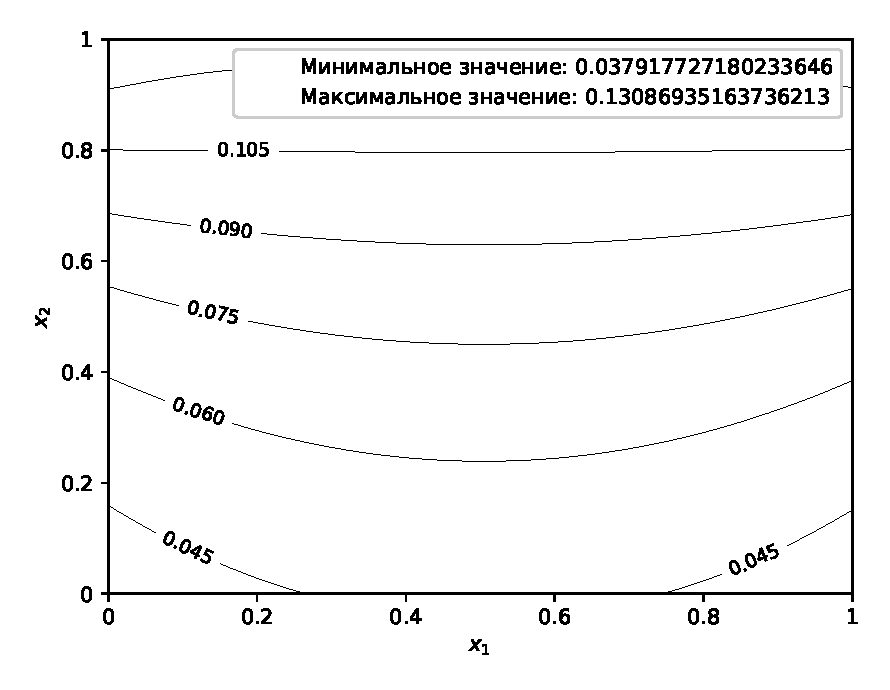
\includegraphics[width=1\linewidth]{boundary/theta_iso_auto} \\ а) $\theta$
    \end{minipage}
    \hfill
    \begin{minipage}[b][][b]{0.49\linewidth}
        \centering
        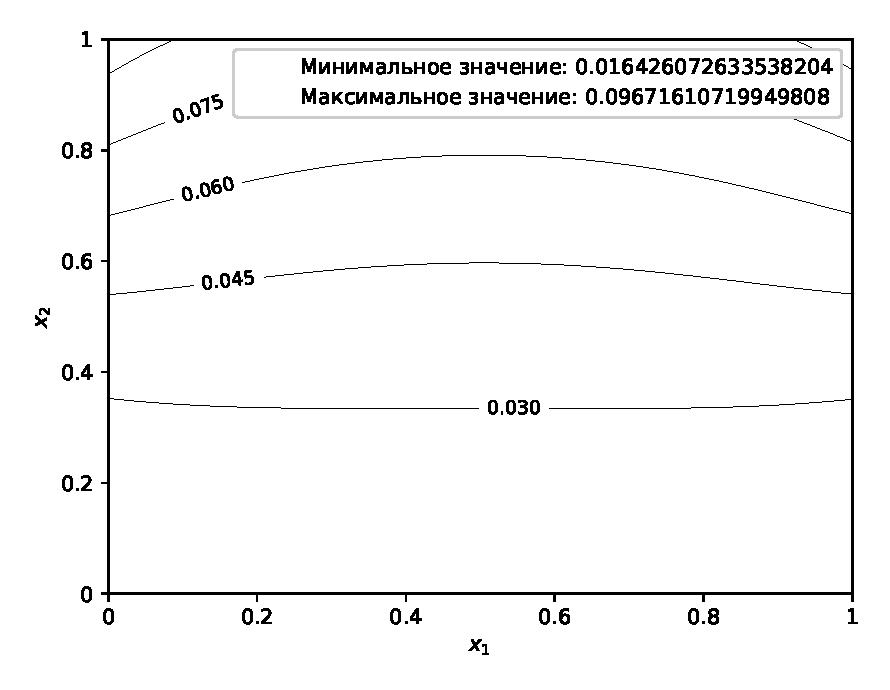
\includegraphics[width=1\linewidth]{boundary/phi_iso_auto} \\ б) $\varphi$
    \end{minipage}
    \caption{Решение граничной задачи в двумерной области}
    \label{fig:4_1:boundary}
\end{figure}


Код, используемый для получения решения представлен в приложении~\ref{lst:boundary}.
Инструментарий для получения изображений можно найти в репозитории~\cite{mesenev-github}.

\textbf{Пример 2} (трёхмерная область).
Пусть $\Omega=\{(x,y,z),\, 0 \leq x,y,z \leq 1 \}$.
Определим функции $\gamma, \theta_b$ следующим образом:
$\gamma = 0.8 \cos\left(\frac{\pi}{2} z\right) + 0.5$,
$\theta_b = 1- y / 2 + z /2$.

Начальное приближение также выберем нулевым.
Для нахождения состояния потребовалось шесть итераций,
результат представлен на рисунке~\ref{fig:4_1:boundary_3d}.
\begin{figure}[h!t]
    \begin{minipage}[b][][b]{0.49\linewidth}
        \centering
        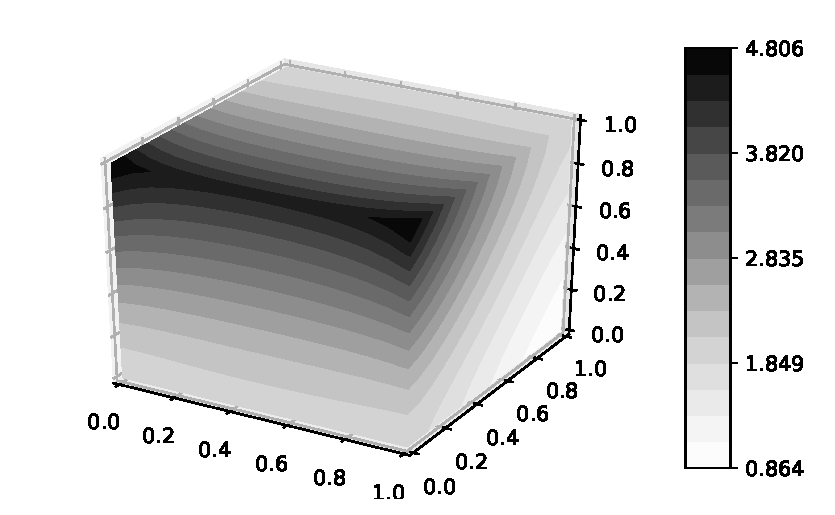
\includegraphics[width=1\linewidth]{boundary/theta_3d} \\ а) $\theta$
    \end{minipage}
    \hfill
    \begin{minipage}[b][][b]{0.49\linewidth}
        \centering
        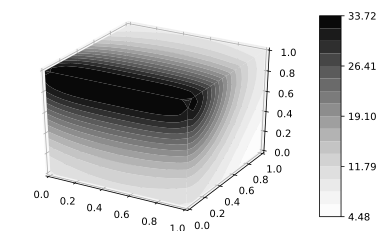
\includegraphics[width=1\linewidth]{boundary/phi_3d} \\ б) $\varphi$
    \end{minipage}
    \caption{Решение граничной задачи в трёхмерной области}
    \label{fig:4_1:boundary_3d}
\end{figure}

\begin{remark}
    Алгоритмы численного решения начально-краевых задач для квазилинейных моделей
    также основаны на предложенном выше методе Ньютона и будут изложены при описании
    алгоритмов решения обратных задач.
\end{remark}

\subsection{Зависимость температурного поля от граничных параметров $\gamma, \beta$}
\label{subsec:ch4/sec1/gamma_beta}


Для исследования зависимости температурного поля от граничных параметров положим
область $\Omega$ равную единичному квадрату.
Параметры среды и граничную функцию $\theta_b$ положим равными
$a = 0.6$, $\alpha = 0.333$, $\kappa_a = 1$, $b = 0.025$, $\beta = 1$
(\textit{параметры среды аналогичны предыдущему примеру и соответствуют параметрам стекла}),
$\theta_b = y$.
Проследим динамику поля температуры
в центральной точке квадрата в зависимости от
изменения граничных параметров $\gamma$ и $\beta$.

\begin{figure}[h!t]
    \begin{minipage}[b][][b]{0.49\linewidth}
        \centering
        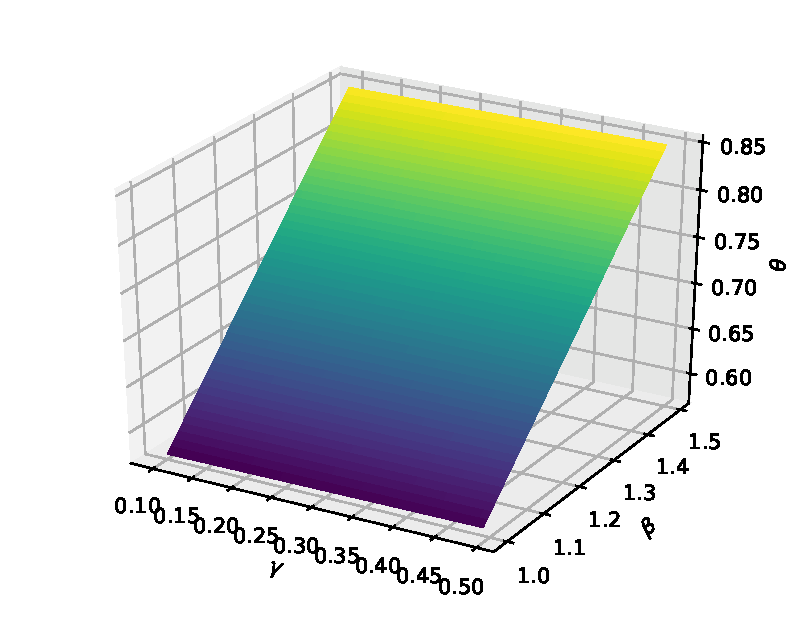
\includegraphics[width=1\linewidth]{additional/1/theta_dynamic}
    \end{minipage}
    \hfill
    \begin{minipage}[b][][b]{0.49\linewidth}
        \centering
        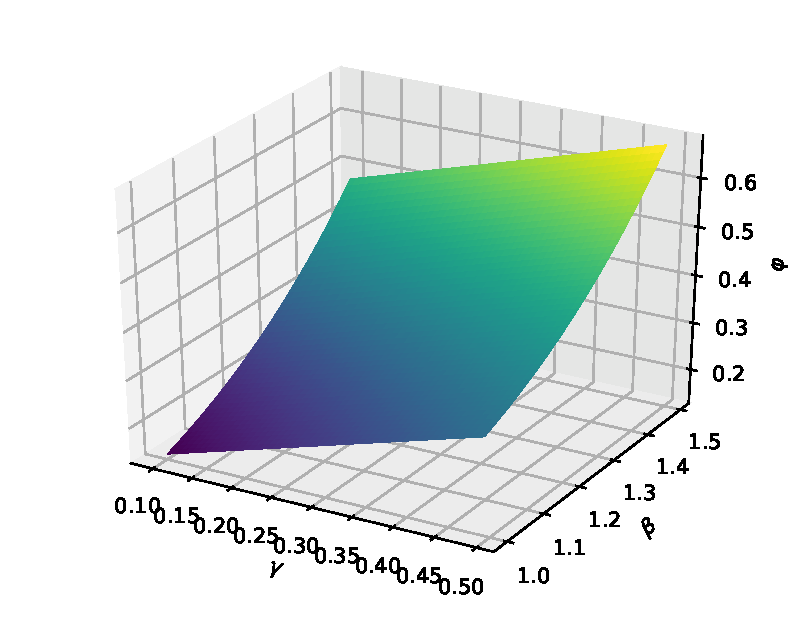
\includegraphics[width=1\linewidth]{additional/1/phi_dynamic}
    \end{minipage}
    \caption{$\theta, \varphi$ в точке $\{0.5, 0.5\}$}
    \label{fig:4_1:dep}
\end{figure}

Рисунок~\ref{fig:4_1:dep} иллюстрирует тот факт, что параметр $\gamma$ оказывает существенно меньшее влияние
на температурное поле, чем параметр $\beta$.
В то же самое время, поле излучения $\varphi$ меняется довольно существенно.
Следовательно, при увеличении параметров $\kappa$ и $b$
будет увеличиваться влияние параметра $\gamma$ на температурное поле $\theta$.
В целях демонстрации положим $b = 1$ и приведём изолинии температурного поля для значений
$\gamma = \{0.1, 0.9\}$.
Как видно из приведённых рисунков~\ref{fig:4_1:theta_diff} температурное поле
в таком случае меняется весьма значительно.
Моделирование в трёхмерной области даёт аналогичные результаты.

\begin{figure}[h!t]
    \begin{minipage}[b][][b]{0.49\linewidth}
        \centering
        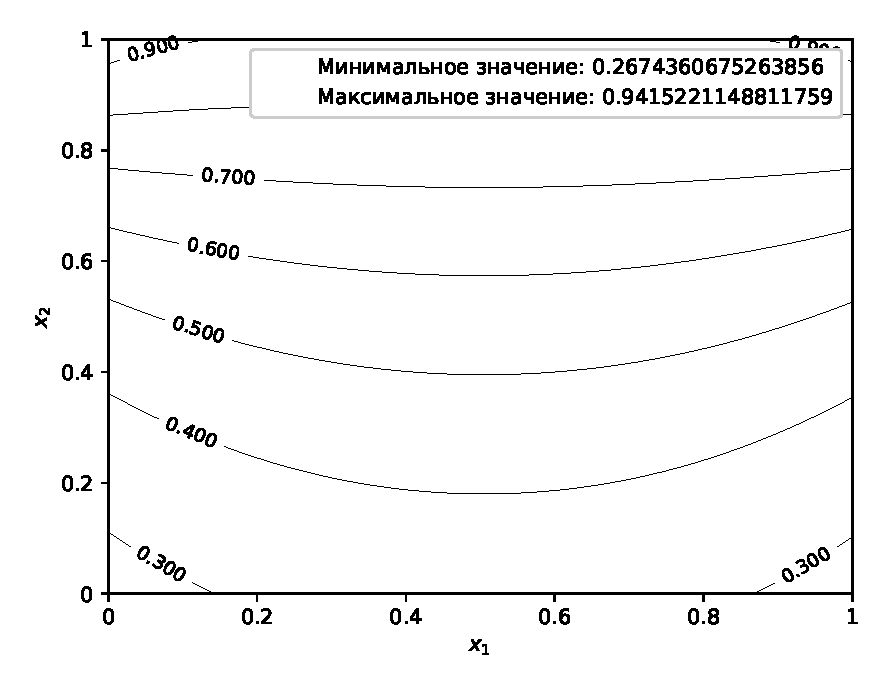
\includegraphics[width=1\linewidth]{additional/1/theta_1_auto} \\ а) $\gamma = 0.1$,
    \end{minipage}
    \hfill
    \begin{minipage}[b][][b]{0.49\linewidth}
        \centering
        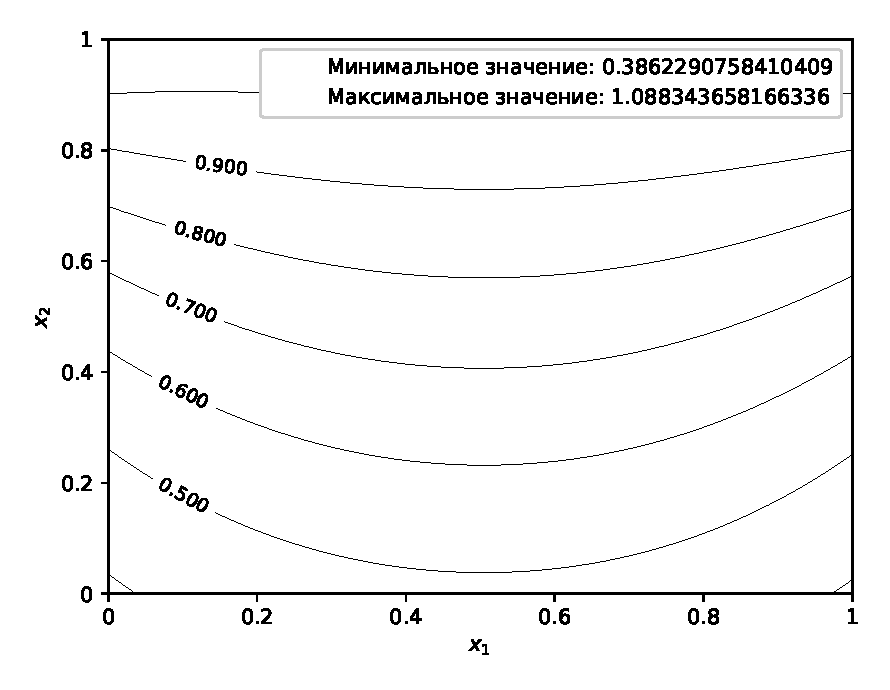
\includegraphics[width=1\linewidth]{additional/1/theta_2_auto} \\ б) $\gamma = 0.9$.
    \end{minipage}
    \caption{$\theta$ при разных значениях параметра $\gamma$.}
    \label{fig:4_1:theta_diff}
\end{figure}

\subsection{Численное решение квазилинейной начально-краевой задачи}
\label{subsec:ch4/sec1/quasilinear}
Моделирование тепла и излучения с параметром среды, зависящим от температуры
имеет множество применений, в том числе, при моделировании медицинских процедур,
использующих высокие температуры.

При расчёте параметров важно учесть характер модели -- её корректность, устойчивость,
область применимости.

Прежде всего нас интересует сходимость модели к устойчивому
решению с течением времени (стабилизация решения).

Рассмотрим начально-краевую задачу~\eqref{eq:1_6:1}--\eqref{eq:1_6:3},
поставленную в разделе~\ref{subsec:ch1/sec5/subsec1}.

Перепишем указанную модель в операторном виде
\begin{equation}
    \label{eq:4_1:nonst_op}
    \begin{gathered}
        \sigma \theta' + A_1(\theta) + b([\theta]^4 - \varphi) = f_b + f, \, \theta(0) = \theta_0 \\
        A_2\varphi + \beta(\varphi - [\theta]^4) = g_b + g.
    \end{gathered}
\end{equation}

Дискретизируя рассматриваемый временной интервал можно установить равенства
$\theta_n \approx \theta(t_n), \varphi_n = \varphi(t_n)$, где $t_n \in [0, T]$.
Производную по времени $\theta'_n$ аппроксимируем как
$\theta'_{n} \approx \frac{\theta_{n} - \theta_{n-1}}{\tau}$.
Здесь $\tau$ параметр дискретизации, $t_n = t_{n-1} + \tau$.
Таким образом, $\varphi_n$ будем искать как решение линейной эллиптической краевой задачи
\[
    A_2 \varphi_n + \beta \varphi_n = \beta [\theta_n]^4 + g_b + g.
\]
Рассчитываем $\theta_{n+1}$ используя следующее равенство
\begin{equation}
    \label{eq:4_1:theta_progress}
    \sigma \theta_{n+1} = \sigma \theta_n - \tau (A_1(\theta_n + b[\theta_n]^4 - \varphi_n) - f_b -f).
\end{equation}

Через моделирование источников излучения $g_b(t)$ и $g(t)$ можно отследить динамику системы и замерить
интересующие параметры при моделировании медицинских процедур внутривенной лазерной абляции.

Полагая $\theta_0 \approx 0$, $f, f_b, g_b, g = 0$, параметры среды определим как
$\alpha = 0.333$,
$ka = 1$,
$b = 0.025$,
$\beta = 1$,
$\gamma = 1$.
Алгоритм расчёта квазилинейной задачи осуществляется итерациями по $n = 1,\dots, N$, $\tau = T/N$,
$\theta_0$ есть начальное распределение температуры.

\begin{remark}
Отметим, что согласно~\eqref{eq:4_1:theta_progress},
параметр $\sigma$ играет роль скорости изменения температурного поля $\theta$, следовательно,
имеет смысл выбирать его обратно пропорциональным параметру $\tau$,
контролируя таким образом скорость моделируемой реакции и количество итераций $N$.
В данном случае в обоих примерах использовались значения $\tau = 1/1200, \sigma = 2$.
Данный подход позволяет учесть условную
устойчивость явной схемы при решении
нестационарной и нелинейной задачи.
\end{remark}

\textbf{Эксперимент 1}.
Параметр $k$ определим как
\[
    k(\theta)=
    \begin{cases}
        0.1, & \text { если } \theta \leq \theta_{*}, \\
        1, & \text { если } \theta>\theta_{*}.
    \end{cases}
\]
Также определим $\theta_b = 1$ на всей границе.
В данном случае $\theta_{*}$ выполняет роль некоторого порогового значения.
Динамика температурного поля в зависимости от выбора $\theta_*$ приведена
на рисунке~\ref{fig:4_1:theta_dyn_diff}а.



\textbf{Эксперимент 2}.
Положим $\theta_b = (x + y) /2$ и
\[
    k(\theta)=
    \begin{cases}
        0.1, & \text { если } \theta \leq 0.5, \\
        m_1, & \text { если } \theta > 0.5.
    \end{cases}
\]

\begin{figure}[h!t]
    \begin{minipage}[b][][b]{0.49\linewidth}
        \centering
        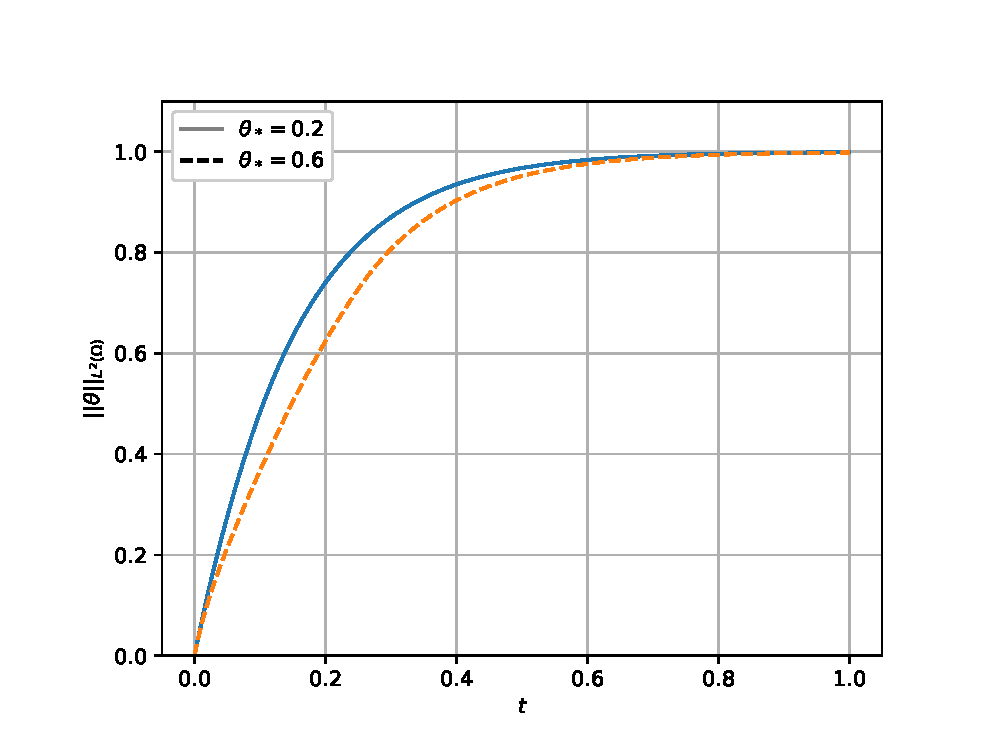
\includegraphics[width=1\linewidth]{additional/3/theta_dyn_star} \\ а) Первый эксперимент
    \end{minipage}
    \hfill
    \begin{minipage}[b][][b]{0.49\linewidth}
        \centering
        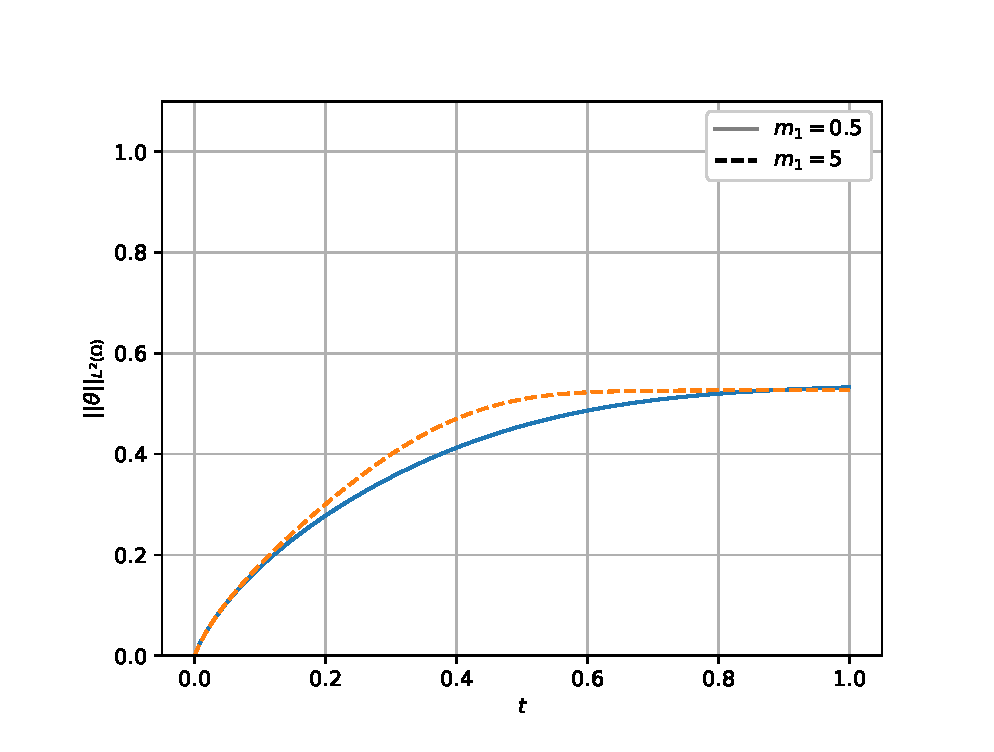
\includegraphics[width=1\linewidth]{additional/3/theta_dyn_m} \\ б) Второй эксперимент
    \end{minipage}
    \caption{Влияние параметра $k(\theta)$ на норму температурного поля.}
    \label{fig:4_1:theta_dyn_diff}
\end{figure}

$k(\theta)$ может оказывать существенное влияние на динамику температурного поля.
На рисунке~\ref{fig:4_1:theta_iso_2exp} приведены изолинии $\theta(T)$,
получившиеся в результате второго эксперимента.
Как видно из изображений, параметр $k$ существенно влияет на распределение температуры.
\begin{figure}[h!t]
    \begin{minipage}[b][][b]{0.49\linewidth}
        \centering
        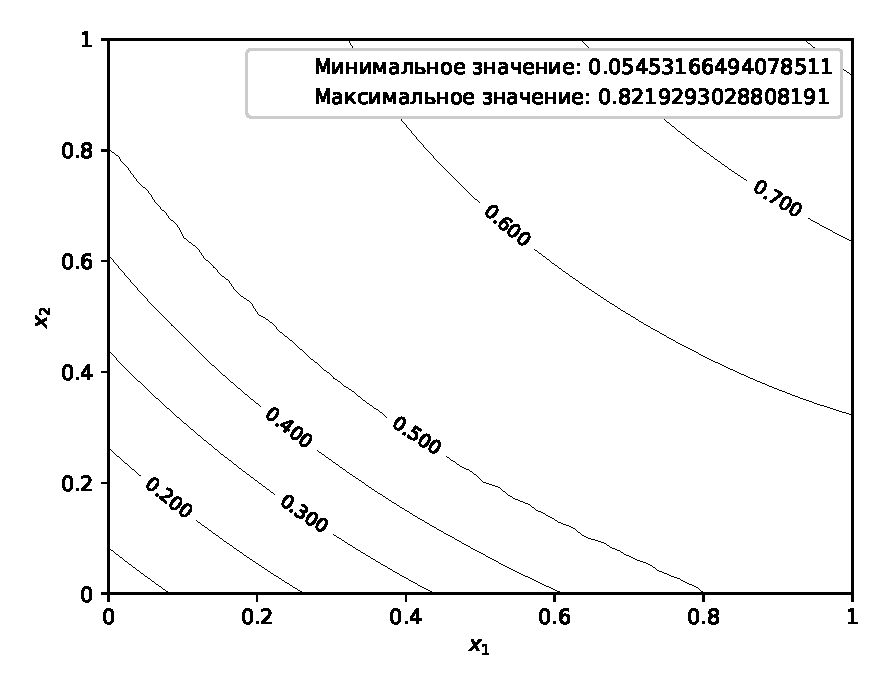
\includegraphics[width=1\linewidth]{additional/3/theta_iso_1} \\ а) $m_1 = 0.5$,
    \end{minipage}
    \hfill
    \begin{minipage}[b][][b]{0.49\linewidth}
        \centering
        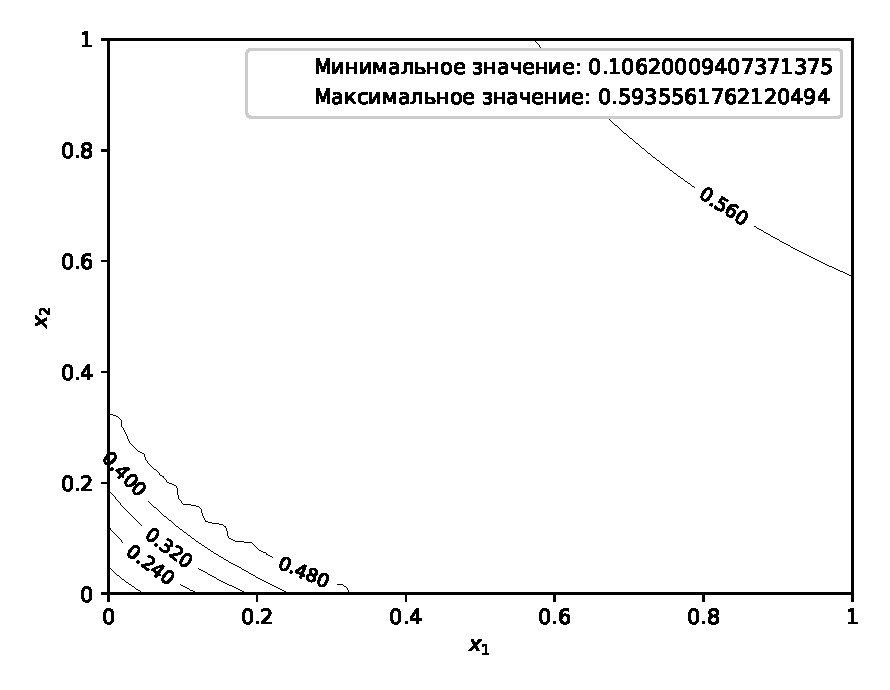
\includegraphics[width=1\linewidth]{additional/3/theta_iso_2} \\ б) $m_1 = 5$.
    \end{minipage}
    \caption{Температурное поле $\theta(T)$}
    \label{fig:4_1:theta_iso_2exp}
\end{figure}


Несмотря на отсутствие соответствующего теоретического обоснования,
полученные результаты численного моделирования
позволяют говорить о стабилизации решения квазилинейной задачи с течением времени.
На рисунке~\ref{fig:4_3:time_diff} показан модуль разности температурных полей
между итерациями для первого эксперимента.
Динамика разности температурного поля по времени в других поставленных экспериментах аналогичная.
\begin{figure}[h!t]
    \begin{minipage}[b][][b]{0.49\linewidth}
        \centering
        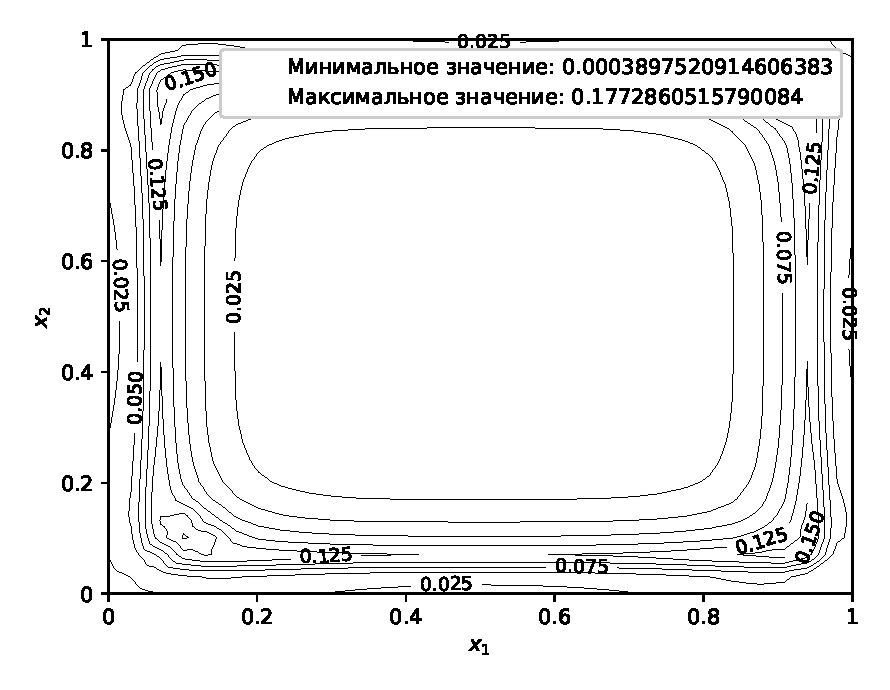
\includegraphics[width=1\linewidth]{additional/3/iso_theta1-theta2_auto} \\ а) $|\theta|_{t=2} - \theta|_{t=3}|$,
    \end{minipage}
    \hfill
    \begin{minipage}[b][][b]{0.49\linewidth}
        \centering
        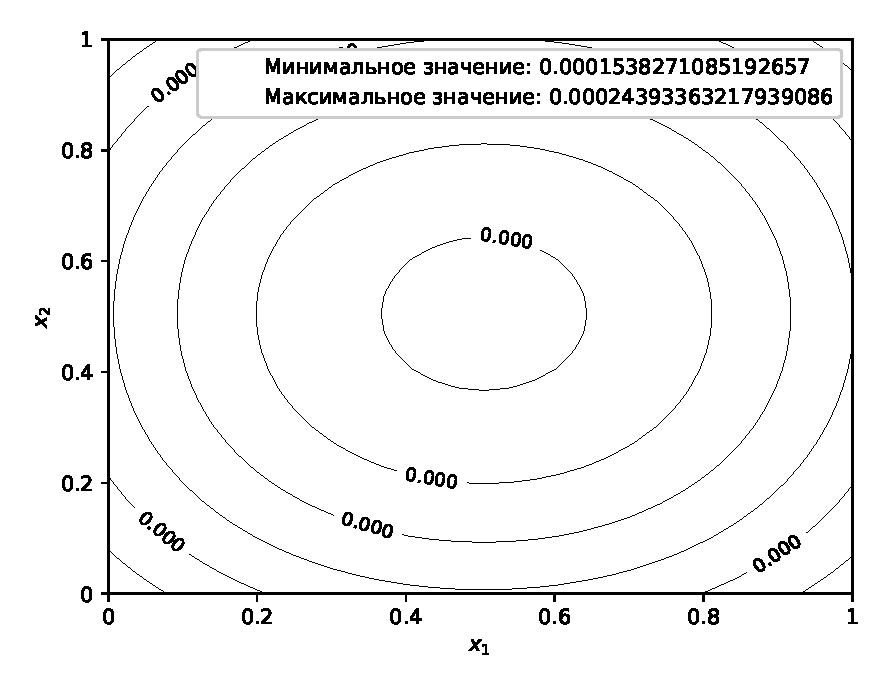
\includegraphics[width=1\linewidth]{additional/3/iso_theta499-theta500_auto} \\ б) $|\theta|_{t=99} - \theta|_{t=100}|$.
    \end{minipage}
    \caption{Модуль разности $\theta$ по итерациям.}
    \label{fig:4_3:time_diff}
\end{figure}


Полученные анимации, а также соответствующий код
экспериментов можно найти по ссылке~\cite{mesenev-github}.


\textbf{Вывод.}
Разработанный численный алгоритм и обширное численное моделирование
(часть результатов которого здесь приведена)
позволяют сделать вывод о значительном влиянии зависимости
коэффициента теплопроводности на процесс, что видимо можно
использовать для моделирования эффектов конвекции.
Влияние на поле излучения оказывается существенным как в скорости сходимости,
так и в конечном распределении температуры в моделируемой области.
Кроме того, численное моделирование с различными параметрами
демонстрирует стабилизацию решения квазилинейной задачи сложного теплообмена.

